% Provenance (never printed): cycle 3 "La planete Terre. Les etres vivants
% dans leur environnement" (natural phenomena: volcanoes and earthquakes,
% natural hazards and the behaviour to adopt); see sources/book1/PROVENANCE.md.
% Book 1, grade 4, chapter 2.
\chapter{ज्वालामुखी और भूकंप: पहली झलक}\label{ch:g4:volcanoes-earthquakes-first-look}

सोमवार शाम समाचार में दूर के एक द्वीप का \omterm{def:g4:volcanoes-earthquakes-first-look:volcano}{ज्वालामुखी} दिखाया जाता है। अँधेरे में
ज़मीन की एक दरार से दमकती नारंगी \omterm{def:g3:stones-pebbles-sand:rock}{चट्टान} का फव्वारा फूटता है, और आग की \omterm{def:g1:landscapes-around-us:water}{नदियाँ}
ढलान पर धीरे-धीरे बहती हुई \omterm{def:g2:water-on-earth:ocean}{समुद्र} में उतरती हैं, सनसनाती और भाप छोड़ती हुई।
गुरुवार को समाचार में एक दूसरी जगह दिखती है: एक छोटा शहर, जहाँ भोर में आधे
मिनट तक ज़मीन काँपती रही। चिमनियाँ गिरकर सड़क पर आ पड़ीं, और एक पुराना मकान
अपनी नींव से खिसक गया।

दो बहुत अलग घटनाएँ। फिर भी दोनों पृथ्वी के बहुत भीतर से आती हैं, और, जैसा हम
देखेंगे, दोनों दुनिया के कुछ हिस्सों में बाक़ी हिस्सों से कहीं ज़्यादा बार होती
हैं।

\begin{recall}
\omterm{def:g1:landscapes-around-us:landform}{पर्वत}, \omterm{def:g1:landscapes-around-us:landform}{पहाड़ियाँ}, \omterm{def:g1:landscapes-around-us:landform}{घाटियाँ} और \omterm{def:g1:landscapes-around-us:landform}{मैदान} ज़मीन के आकार हैं
(\cref{ch:g1:landscapes-around-us})। पृथ्वी की ज़मीन सात \omterm{def:g3:continents-and-oceans:continent}{महाद्वीपों} में बँटी है,
जो पाँच \omterm{def:g2:water-on-earth:ocean}{महासागरों} के बीच हैं; प्रशांत \omterm{def:g2:water-on-earth:ocean}{महासागर} सबसे बड़ा \omterm{def:g2:water-on-earth:ocean}{महासागर} है
(\cref{ch:g3:continents-and-oceans})।
\end{recall}

\section{एक ज्वालामुखी फूटता है}

हमारे पैरों के बहुत नीचे पृथ्वी बहुत गरम है। कुछ जगहों पर वहाँ नीचे की \omterm{def:g3:stones-pebbles-sand:rock}{चट्टान}
इतनी गरम है कि वह पिघल गई है। यह पिघली \omterm{def:g3:stones-pebbles-sand:rock}{चट्टान} अपने आसपास की ठोस \omterm{def:g3:stones-pebbles-sand:rock}{चट्टान} से
हल्की है, इसलिए वह धीरे-धीरे ऊपर उठती है, जैसे पानी में कॉर्क। जहाँ उसे सतह तक
निकलने का रास्ता मिलता है, वहाँ एक \omterm{def:g4:volcanoes-earthquakes-first-look:volcano}{ज्वालामुखी} जन्म लेता है।

\begin{definition}[ज्वालामुखी]\label{def:g4:volcanoes-earthquakes-first-look:volcano}
\emph{ज्वालामुखी}\index{ज्वालामुखी} वह जगह है जहाँ पृथ्वी के बहुत भीतर की पिघली
\omterm{def:g3:stones-pebbles-sand:rock}{चट्टान} सतह पर निकलती है, और वह \omterm{def:g1:landscapes-around-us:landform}{पहाड़ी} या \omterm{def:g1:landscapes-around-us:landform}{पर्वत} भी जिसे पिघली \omterm{def:g3:stones-pebbles-sand:rock}{चट्टान} वहाँ परत
पर परत बनाती है।
\end{definition}

\begin{definition}[उद्गार, लावा और ज्वालामुखीय राख]\label{def:g4:volcanoes-earthquakes-first-look:eruption}
\emph{उद्गार}\index{उद्गार} वह समय है जब \omterm{def:g4:volcanoes-earthquakes-first-look:volcano}{ज्वालामुखी} पिघली \omterm{def:g3:stones-pebbles-sand:rock}{चट्टान}, राख और गैस बाहर
फेंकता है। \emph{लावा}\index{लावा} वह पिघली \omterm{def:g3:stones-pebbles-sand:rock}{चट्टान} है जो सतह पर उमड़कर बहती
है; वह बहता है, फिर ठंडा होकर कठोर नई \omterm{def:g3:stones-pebbles-sand:rock}{चट्टान} बन जाता है।
\emph{ज्वालामुखीय राख}\index{ज्वालामुखीय राख} \omterm{def:g3:stones-pebbles-sand:rock}{चट्टान} और काँच के नन्हे टुकड़ों से बनी
होती है जिन्हें उद्गार हवा में उड़ा देता है; वह धूसर \omterm{def:g4:clouds-rain-snow:precipitation}{हिम} की तरह वापस गिरती है।
\end{definition}

\begin{omfigure}
\begin{tikzpicture}[font=\small]
  % ground and deep rock
  \fill[brown!30] (-5,-2.6) rectangle (5,0);
  % the volcano
  \fill[black!40] (-4.2,0) -- (-0.6,3.0) -- (0.6,3.0) -- (4.2,0) -- cycle;
  \fill[black!55] (-0.6,3.0) -- (-0.35,2.75) -- (0.35,2.75) -- (0.6,3.0) -- cycle;
  % layers inside the cone
  \foreach \k in {1,2,3}
    \draw[black!25] (-4.2+1.0*\k,0) -- (-0.6+0.05*\k,3.0-0.25*\k);
  % molten rock rising from deep below
  \fill[orange!80!red] (-0.25,-2.6) -- (-0.25,2.75) -- (0.25,2.75) -- (0.25,-2.6) -- cycle;
  \fill[orange!80!red] (0,-2.6) ellipse (1.6 and 0.5);
  % lava flow on the right flank
  \fill[orange!90!red] (0.5,2.9) .. controls (1.2,2.2) and (1.4,1.6) .. (2.2,1.0)
    .. controls (2.6,0.6) and (3.2,0.25) .. (3.7,0.1) -- (3.3,0.1)
    .. controls (2.6,0.35) and (2.0,0.75) .. (1.7,1.1)
    .. controls (1.2,1.6) and (0.9,2.3) .. (0.3,2.9) -- cycle;
  % ash and gas cloud
  \foreach \x/\y/\r in {0/3.6/0.45, -0.5/4.2/0.55, 0.4/4.3/0.5, -0.2/4.9/0.6, 0.6/5.0/0.55, -0.9/4.8/0.45, 0.1/5.5/0.6}
    \fill[black!25] (\x,\y) circle (\r);
  % labels
  \node[anchor=west] at (2.3,5.0) {राख और गैस};
  \draw[black!60] (2.25,5.0) -- (1.1,4.9);
  \node[anchor=west] at (3.3,1.6) {लावा की धारा};
  \draw[black!60] (3.25,1.6) -- (2.1,1.1);
  \node[anchor=east] at (-3.0,2.0) {ज्वालामुखी};
  \draw[black!60] (-2.95,2.0) -- (-1.9,1.5);
  \node[anchor=west, align=left] at (1.9,-1.4) {नीचे गहराई से उठती\\पिघली चट्टान};
  \draw[black!60] (1.85,-1.4) -- (0.3,-1.2);
\end{tikzpicture}

{\small फूटता हुआ \omterm{def:g4:volcanoes-earthquakes-first-look:volcano}{ज्वालामुखी} (चित्र पैमाने पर नहीं)। पिघली \omterm{def:g3:stones-pebbles-sand:rock}{चट्टान} नीचे गहराई से
उठती है और चोटी पर निकलती है: वह \omterm{def:g4:volcanoes-earthquakes-first-look:eruption}{लावा} बनकर नीचे बहती है, जबकि राख और गैस
आसमान में ऊपर उड़ जाती हैं। हर \omterm{def:g4:volcanoes-earthquakes-first-look:eruption}{उद्गार} \omterm{def:g1:landscapes-around-us:landform}{पर्वत} पर एक नई परत जोड़ता है।}
\label{fig:g4:volcanoes-earthquakes-first-look:volcano}
\end{omfigure}

सभी \omterm{def:g4:volcanoes-earthquakes-first-look:eruption}{उद्गार} एक जैसे नहीं दिखते। कुछ में \omterm{def:g4:volcanoes-earthquakes-first-look:eruption}{लावा} पतला होता है: वह दमकती \omterm{def:g1:landscapes-around-us:water}{नदियों} में
चुपचाप उमड़ता है जो किलोमीटरों तक बह सकती हैं, कभी-कभी \omterm{def:g2:water-on-earth:ocean}{समुद्र} तक। दूसरों में
पिघली \omterm{def:g3:stones-pebbles-sand:rock}{चट्टान} गाढ़ी और गैस से भरी होती है, जैसे हिलाई हुई सोडा की बोतल: जब वह
फूटकर निकलती है, तो राख के एक विशाल स्तंभ में फट पड़ती है जो आसमान में बहुत
ऊँचा उठता है।

\begin{omfigure}
\begin{minipage}[b]{0.56\linewidth}\centering
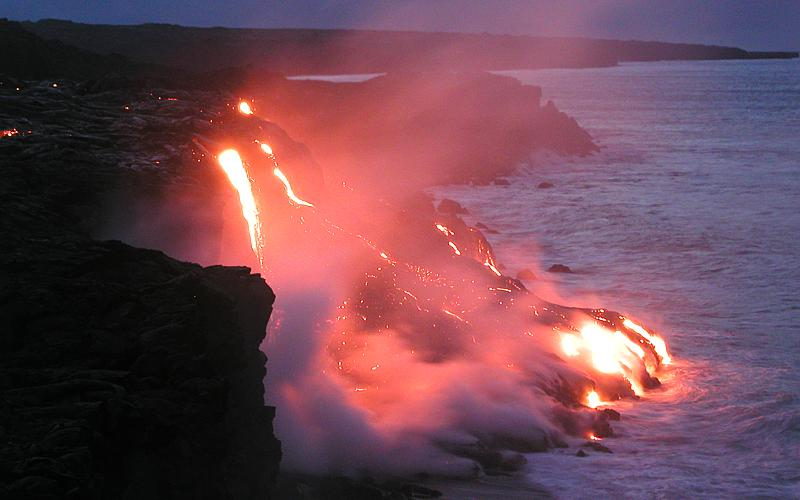
\includegraphics[width=\linewidth]{images/book1/g4-lava-ocean.jpg}

{\small पतला \omterm{def:g4:volcanoes-earthquakes-first-look:eruption}{उद्गार}: हवाई में \omterm{def:g4:volcanoes-earthquakes-first-look:eruption}{लावा} समुद्री कगार से नीचे \omterm{def:g2:water-on-earth:ocean}{महासागर} में गिरता है।
चित्र: USGS हवाई \omterm{def:g4:volcanoes-earthquakes-first-look:volcano}{ज्वालामुखी} वेधशाला (सार्वजनिक डोमेन)।}
\end{minipage}\hfill
\begin{minipage}[b]{0.4\linewidth}\centering
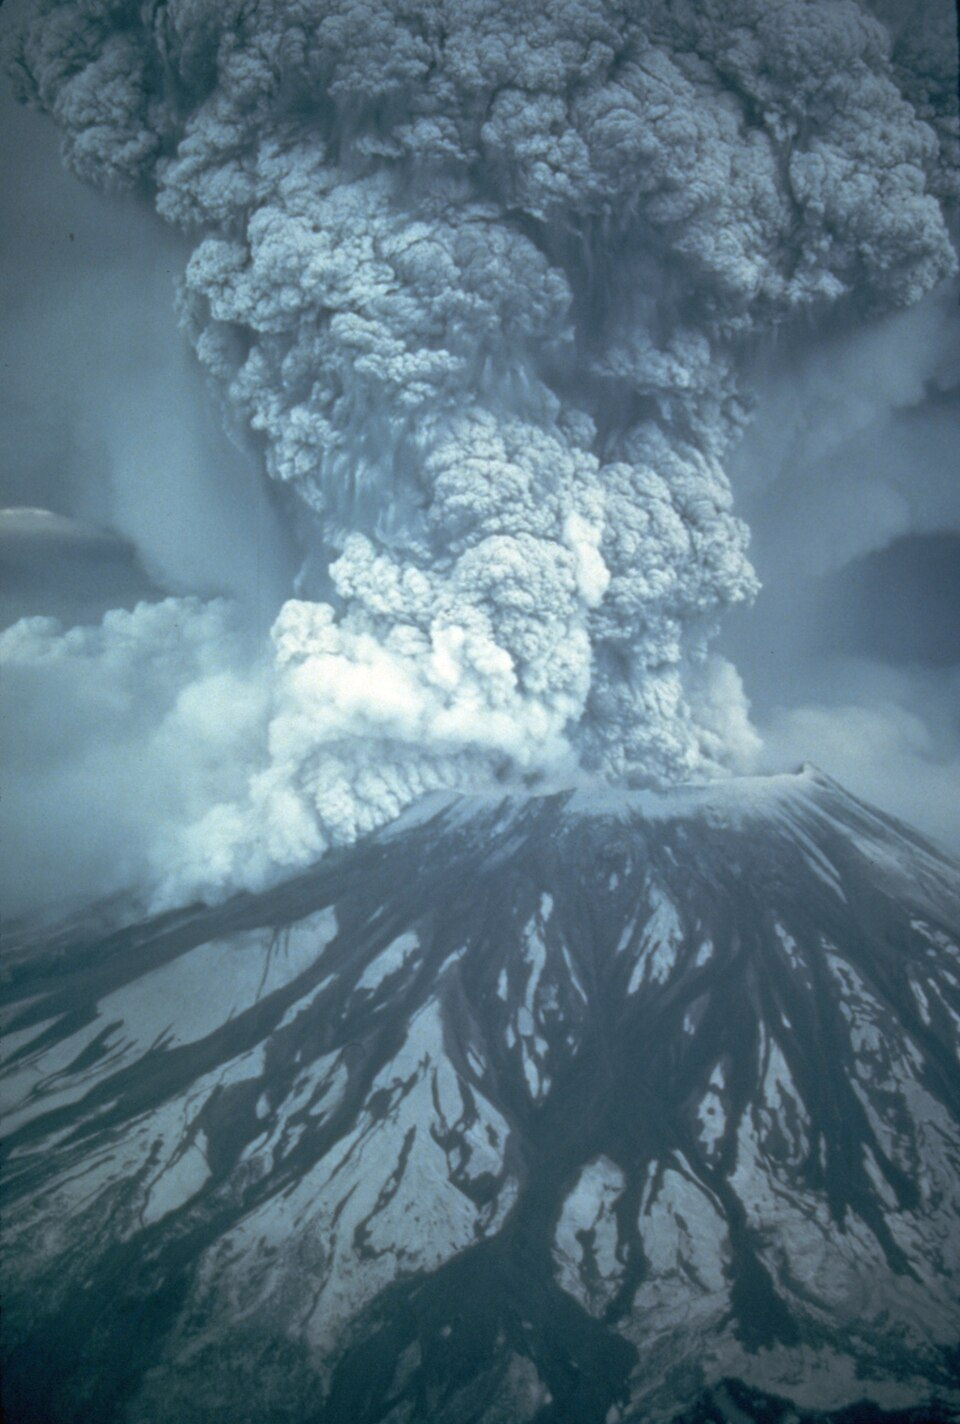
\includegraphics[width=0.78\linewidth]{images/book1/g4-st-helens.jpg}

{\small विस्फोटक \omterm{def:g4:volcanoes-earthquakes-first-look:eruption}{उद्गार}: माउंट सेंट~हेलेंस, संयुक्त राज्य अमेरिका, 18~मई 1980।
चित्र: ऑस्टिन पोस्ट, USGS (सार्वजनिक डोमेन)।}
\end{minipage}
% ledger: usgs:pu-oo-ocean, usgs:msh-1980
\label{fig:g4:volcanoes-earthquakes-first-look:two-eruptions}
\end{omfigure}

\begin{example}[माउंट सेंट~हेलेंस, 1980]\label{ex:g4:volcanoes-earthquakes-first-look:st-helens}
1980 के वसंत में माउंट सेंट~हेलेंस की बगल में एक उभार बढ़ने लगा, क्योंकि पिघली
\omterm{def:g3:stones-pebbles-sand:rock}{चट्टान} \omterm{def:g1:landscapes-around-us:landform}{पर्वत} के भीतर ऊपर की ओर धकेल रही थी। 18~मई की सुबह एक छोटे \omterm{def:g4:volcanoes-earthquakes-first-look:earthquake}{भूकंप} ने
\omterm{def:g1:landscapes-around-us:landform}{पर्वत} को हिलाया, उभार एक विशाल भूस्खलन में खिसक गया, और \omterm{def:g4:volcanoes-earthquakes-first-look:volcano}{ज्वालामुखी} बगल की ओर
और ऊपर की ओर फट पड़ा। \omterm{def:g1:landscapes-around-us:landform}{पर्वत} का ऊपरी 400~मीटर हिस्सा ग़ायब हो गया: चोटी एक
विशाल गड्ढा बन गई।
% ledger: usgs:msh-1980
\end{example}

\section{ज़मीन काँपती है}

हमारे पैरों के बहुत नीचे की \omterm{def:g3:stones-pebbles-sand:rock}{चट्टानें} पूरी तरह स्थिर नहीं हैं। बहुत धीरे-धीरे
उन्हें धकेला और खींचा जाता है। वे थोड़ा मुड़ती हैं, उस पैमाने की तरह जिसे तुम
दोनों सिरों से दबाते हो --- जब तक कि अचानक वे टूटकर खिसक नहीं जातीं। यह झटका
चारों ओर किलोमीटरों तक ज़मीन को कँपा देता है।

\begin{definition}[भूकंप]\label{def:g4:volcanoes-earthquakes-first-look:earthquake}
\emph{भूकंप}\index{भूकंप} ज़मीन का अचानक काँपना है, जो ज़मीन के बहुत नीचे टूटती
और खिसकती \omterm{def:g3:stones-pebbles-sand:rock}{चट्टानों} के कारण होता है।
\end{definition}

\omterm{def:g4:volcanoes-earthquakes-first-look:earthquake}{भूकंप} आमतौर पर कुछ ही सेकंड चलता है, सबसे बड़े \omterm{def:g4:volcanoes-earthquakes-first-look:earthquake}{भूकंपों} में कभी-कभी एक-दो मिनट।
ज़्यादातर \omterm{def:g4:volcanoes-earthquakes-first-look:earthquake}{भूकंप} इतने छोटे होते हैं कि उन्हें कोई महसूस नहीं करता: केवल यंत्र
उन्हें पकड़ते हैं। एक तेज़ \omterm{def:g4:volcanoes-earthquakes-first-look:earthquake}{भूकंप} ज़मीन को जहाज़ के डेक की तरह लहरा सकता है,
सड़कों में दरारें डाल सकता है, और दीवारें और मकान गिरा सकता है।

\begin{omfigure}
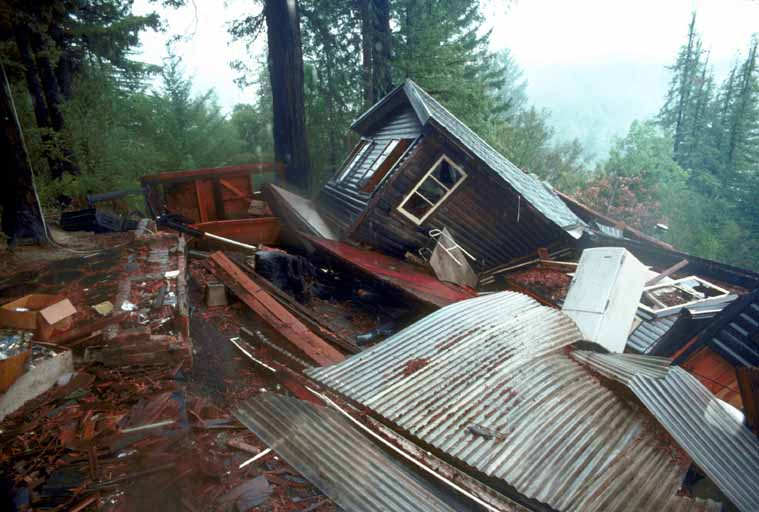
\includegraphics[width=0.55\linewidth]{images/book1/g4-loma-prieta-house.jpg}

{\small कैलिफ़ोर्निया में 1989 के एक तेज़ \omterm{def:g4:volcanoes-earthquakes-first-look:earthquake}{भूकंप} के बाद: यह लकड़ी का मकान अपनी
कंक्रीट की नींव से बगल में फेंक दिया गया। चित्र: नकाटा, USGS
(सार्वजनिक डोमेन)।}
% ledger: usgs:loma-prieta-house
\end{omfigure}

\begin{remark}[कितनी बार?]\label{rem:g4:volcanoes-earthquakes-first-look:how-often}
भूवैज्ञानिक पृथ्वी के सभी बड़े \omterm{def:g4:volcanoes-earthquakes-first-look:earthquake}{भूकंपों} की एक सूची रखते हैं। 1976 से 2025 तक के
50 वर्षों में इस सूची में 7\,031 बड़े \omterm{def:g4:volcanoes-earthquakes-first-look:earthquake}{भूकंप} गिने गए (इतने तेज़ कि पास की इमारतों
को नुक़सान पहुँचा सकें): साल में लगभग 141, यानी हर हफ़्ते लगभग 3। सबसे बड़े
\omterm{def:g4:volcanoes-earthquakes-first-look:earthquake}{भूकंप}, जो पूरे शहर नष्ट कर सकते हैं, साल में लगभग 14 होते हैं। इसी पृथ्वी पर
पिछले लगभग बारह हज़ार वर्षों में लगभग 1\,200 \omterm{def:g4:volcanoes-earthquakes-first-look:volcano}{ज्वालामुखी} फूट
चुके हैं।
% ledger: data:usgs-comcat, data:gvp
\end{remark}

\section{ज्वालामुखी और भूकंप कहाँ होते हैं}

अगर \omterm{def:g4:volcanoes-earthquakes-first-look:volcano}{ज्वालामुखी} और \omterm{def:g4:volcanoes-earthquakes-first-look:earthquake}{भूकंप} कहीं भी बेतरतीब ढंग से होते, तो \omterm{def:g3:continents-and-oceans:world-map}{विश्व मानचित्र} पर उनके
बिंदु उस पर बराबर छिटके होते। ऐसा नहीं है।

नीचे का \omterm{def:g2:drawing-to-map:map}{मानचित्र} एक चौंकाने वाला पैटर्न दिखाता है। ज़्यादातर \omterm{def:g4:volcanoes-earthquakes-first-look:volcano}{ज्वालामुखी} और
ज़्यादातर बड़े \omterm{def:g4:volcanoes-earthquakes-first-look:earthquake}{भूकंप} लंबी, सँकरी पट्टियों में हैं। सबसे लंबी पट्टी प्रशांत
\omterm{def:g2:water-on-earth:ocean}{महासागर} के चारों ओर जाती है: न्यूज़ीलैंड से ऊपर इंडोनेशिया, फ़िलीपींस और जापान
होकर, पार अलास्का तक, फिर अमेरिका महाद्वीपों के पश्चिमी \omterm{def:g1:landscapes-around-us:water}{तट} के साथ-साथ नीचे
चिली के छोर तक। अपने बहुत-से \omterm{def:g4:volcanoes-earthquakes-first-look:volcano}{ज्वालामुखियों} के कारण इसे अक्सर ``अग्नि-वलय''
कहा जाता है।

\begin{example}[मानचित्र पर गिनती]\label{ex:g4:volcanoes-earthquakes-first-look:shares}
हमने वे बिंदु गिने जो छायांकित वलय में पड़ते हैं, यानी उसकी बीच की रेखा
से 500~किलोमीटर के भीतर। 1\,214 \omterm{def:g4:volcanoes-earthquakes-first-look:volcano}{ज्वालामुखियों} में से 837 वलय में हैं: हर 3 में से
लगभग 2। 696 बहुत बड़े \omterm{def:g4:volcanoes-earthquakes-first-look:earthquake}{भूकंपों} में से 532 वलय में हैं: हर 4 में से लगभग 3। वलय
पृथ्वी का केवल एक छोटा हिस्सा घेरता है, पर उसमें पृथ्वी के ज़्यादातर \omterm{def:g4:volcanoes-earthquakes-first-look:volcano}{ज्वालामुखी}
और \omterm{def:g4:volcanoes-earthquakes-first-look:earthquake}{भूकंप} हैं।
% ledger: data:gvp, data:usgs-comcat
\end{example}

\begin{omfigure}
\begin{tikzpicture}
\begin{axis}[ommap, width=\linewidth, xtick=\empty, ytick=\empty, grid=none,
    legend style={font=\scriptsize, at={(0.5,-0.02)}, anchor=north,
      draw=none, legend columns=3, /tikz/every even column/.append style={column sep=6pt}},
    legend cell align=left]
  \addplot[fill=omHypsLandA!85!black, draw=black!45, line width=0.2pt, forget plot]
    table {figdata/out/shared-geo-land.dat};
  \addplot[orange!80!black, opacity=0.35, line width=9pt, line cap=round, line join=round]
    table {figdata/out/grade-4-ring_of_fire-ring.dat};
  \addlegendentry{प्रशांत के चारों ओर का वलय}
  \addplot[only marks, mark=triangle*, mark size=1.3pt, red!75!black]
    table[x=lon, y=lat] {figdata/out/grade-4-ring_of_fire-volcanoes.dat};
  \addlegendentry{एक ज्वालामुखी (पिछले 12\,000 वर्ष)}
  \addplot[only marks, mark=*, mark size=1.0pt, black, fill opacity=0.6]
    table[x=lon, y=lat] {figdata/out/grade-4-ring_of_fire-quakes7.dat};
  \addlegendentry{एक बहुत बड़ा भूकंप (1976--2025)}
\end{axis}
\end{tikzpicture}

{\small पिछले लगभग बारह हज़ार वर्षों में फूटे \omterm{def:g4:volcanoes-earthquakes-first-look:volcano}{ज्वालामुखी}, और 1976--2025 के सबसे
बड़े \omterm{def:g4:volcanoes-earthquakes-first-look:earthquake}{भूकंप}। उनमें से ज़्यादातर प्रशांत \omterm{def:g2:water-on-earth:ocean}{महासागर} के चारों ओर द्वीप-शृंखलाओं और
पर्वत-मालाओं के एक वलय (छायांकित) के साथ-साथ हैं। आँकड़े: स्मिथसोनियन ग्लोबल
वोल्कैनिज़्म प्रोग्राम; अमेरिकी भूवैज्ञानिक सर्वेक्षण की भूकंप-सूची; तटरेखाएँ
नैचुरल अर्थ।}
\label{fig:g4:volcanoes-earthquakes-first-look:map}
% ledger: data:gvp, data:usgs-comcat, data:ne-land
\end{omfigure}

दूसरी पट्टियाँ छोटी हैं: एक दक्षिणी यूरोप और एशिया को पार करती है, भूमध्य सागर
से हिमालय तक; दूसरी \omterm{def:g2:water-on-earth:ocean}{महासागरों} के बीचोंबीच नीचे की ओर जाती हैं, जहाँ \omterm{def:g4:volcanoes-earthquakes-first-look:volcano}{ज्वालामुखी}
पानी के नीचे छिपे हैं। कुछ जगहों पर, जैसे हवाई में, किसी भी पट्टी से दूर
\omterm{def:g4:volcanoes-earthquakes-first-look:volcano}{ज्वालामुखी} हैं। पट्टियाँ जहाँ हैं वहीं क्यों हैं, यह \cref{ch:g7:plate-tectonics} का प्रश्न है:
इसका जवाब पूरे \omterm{def:g2:drawing-to-map:map}{मानचित्र} का आकार समझाता है।

\section{सुरक्षित रहना}

कोई \omterm{def:g4:volcanoes-earthquakes-first-look:eruption}{उद्गार} या \omterm{def:g4:volcanoes-earthquakes-first-look:earthquake}{भूकंप} को रोक नहीं सकता। पर यह जानना कि क्या करना है, जानें
बचाता है।

\begin{omfigure}
\begin{tikzpicture}[font=\small, line cap=round, line join=round]
  % --- panel 1: DROP onto hands and knees
  \begin{scope}
    \draw[black!30] (-0.2,0) -- (2.8,0);
    \fill[omDef] (0.62,0.98) circle (0.21);
    \draw[omDef, line width=2.2pt] (0.88,0.98) -- (2.0,0.95);
    \draw[omDef, line width=2pt] (0.95,0.96) -- (0.95,0.05);
    \draw[omDef, line width=2pt] (2.0,0.95) -- (1.98,0.08) -- (2.65,0.08);
    \node[font=\bfseries] at (1.3,-0.45) {झुको};
    \node[font=\scriptsize, align=center] at (1.3,-1.02) {अपने हाथों और\\घुटनों पर};
  \end{scope}
  % --- panel 2: COVER under a table
  \begin{scope}[xshift=4cm]
    \draw[black!30] (-0.2,0) -- (2.8,0);
    \fill[brown!60!black] (-0.1,1.45) rectangle (2.7,1.6);
    \draw[brown!60!black, line width=2pt] (0.1,1.45) -- (0.1,0) (2.5,1.45) -- (2.5,0);
    \fill[omDef] (0.75,0.95) circle (0.2);
    \draw[omDef, line width=2.2pt] (0.95,0.85) -- (1.95,0.8);
    \draw[omDef, line width=2pt] (1.9,0.8) -- (1.65,0.05) -- (2.25,0.05);
    \draw[omDef, line width=2pt] (1.0,0.85) -- (0.7,1.2) -- (0.5,0.95);
    \node[font=\bfseries] at (1.3,-0.45) {ढको};
    \node[font=\scriptsize, align=center] at (1.3,-1.02) {अपना सिर और गर्दन,\\मज़बूत मेज़ के नीचे};
  \end{scope}
  % --- panel 3: HOLD ON to the table leg
  \begin{scope}[xshift=8cm]
    \draw[black!30] (-0.2,0) -- (2.8,0);
    \fill[brown!60!black] (-0.1,1.45) rectangle (2.7,1.6);
    \draw[brown!60!black, line width=2pt] (0.1,1.45) -- (0.1,0) (2.5,1.45) -- (2.5,0);
    \fill[omDef] (0.75,0.95) circle (0.2);
    \draw[omDef, line width=2.2pt] (0.95,0.85) -- (1.95,0.8);
    \draw[omDef, line width=2pt] (1.9,0.8) -- (1.65,0.05) -- (2.25,0.05);
    \draw[omDef, line width=2pt] (1.0,0.85) -- (0.7,1.2) -- (0.5,0.95);
    \draw[omDef, line width=2pt] (1.0,0.8) -- (0.45,0.6) -- (0.12,0.65);
    \node[font=\bfseries] at (1.3,-0.45) {पकड़े रहो};
    \node[font=\scriptsize, align=center] at (1.3,-1.02) {मेज़ को, जब तक\\काँपना न रुके};
  \end{scope}
\end{tikzpicture}

{\small ज़मीन काँपने लगते ही क्या करें: झुको, ढको और
पकड़े रहो।}
\label{fig:g4:volcanoes-earthquakes-first-look:drop-cover}
% ledger: shakeout:dch
\end{omfigure}

\begin{safety}
\textbf{\omterm{def:g4:volcanoes-earthquakes-first-look:earthquake}{भूकंप} में।} जैसे ही तुम्हें ज़मीन काँपती महसूस हो:
अपने हाथों और घुटनों पर \textbf{झुको}; अपने सिर और गर्दन को बाँह से \textbf{ढको},
और अगर पास में कोई मज़बूत मेज़ या डेस्क हो तो उसके नीचे घुस जाओ;
काँपना रुकने तक उसे \textbf{पकड़े रहो}। जब ज़मीन काँप रही हो तब बाहर मत भागो,
और दरवाज़े की चौखट में खड़े मत हो: गिरता काँच और गिरती चीज़ें
सबसे बड़ा ख़तरा हैं। जब काँपना रुक जाए, तो शांति से इमारत से बाहर निकलो, जैसे
तुम स्कूल की ड्रिलों में करते हो।

\textbf{\omterm{def:g4:volcanoes-earthquakes-first-look:volcano}{ज्वालामुखी} के पास।} वैज्ञानिक उन \omterm{def:g4:volcanoes-earthquakes-first-look:volcano}{ज्वालामुखियों} पर नज़र रखते हैं जो जाग
सकते हैं। अगर वे चेतावनी दें कि \omterm{def:g4:volcanoes-earthquakes-first-look:eruption}{उद्गार} आने वाला है, तो अधिकारी लोगों से वह
इलाक़ा छोड़ने को कहते हैं। उनके निर्देश तुरंत मानो, और देखने के लिए कभी पास मत जाओ।
\end{safety}
% ledger: shakeout:dch

\begin{omfigure}
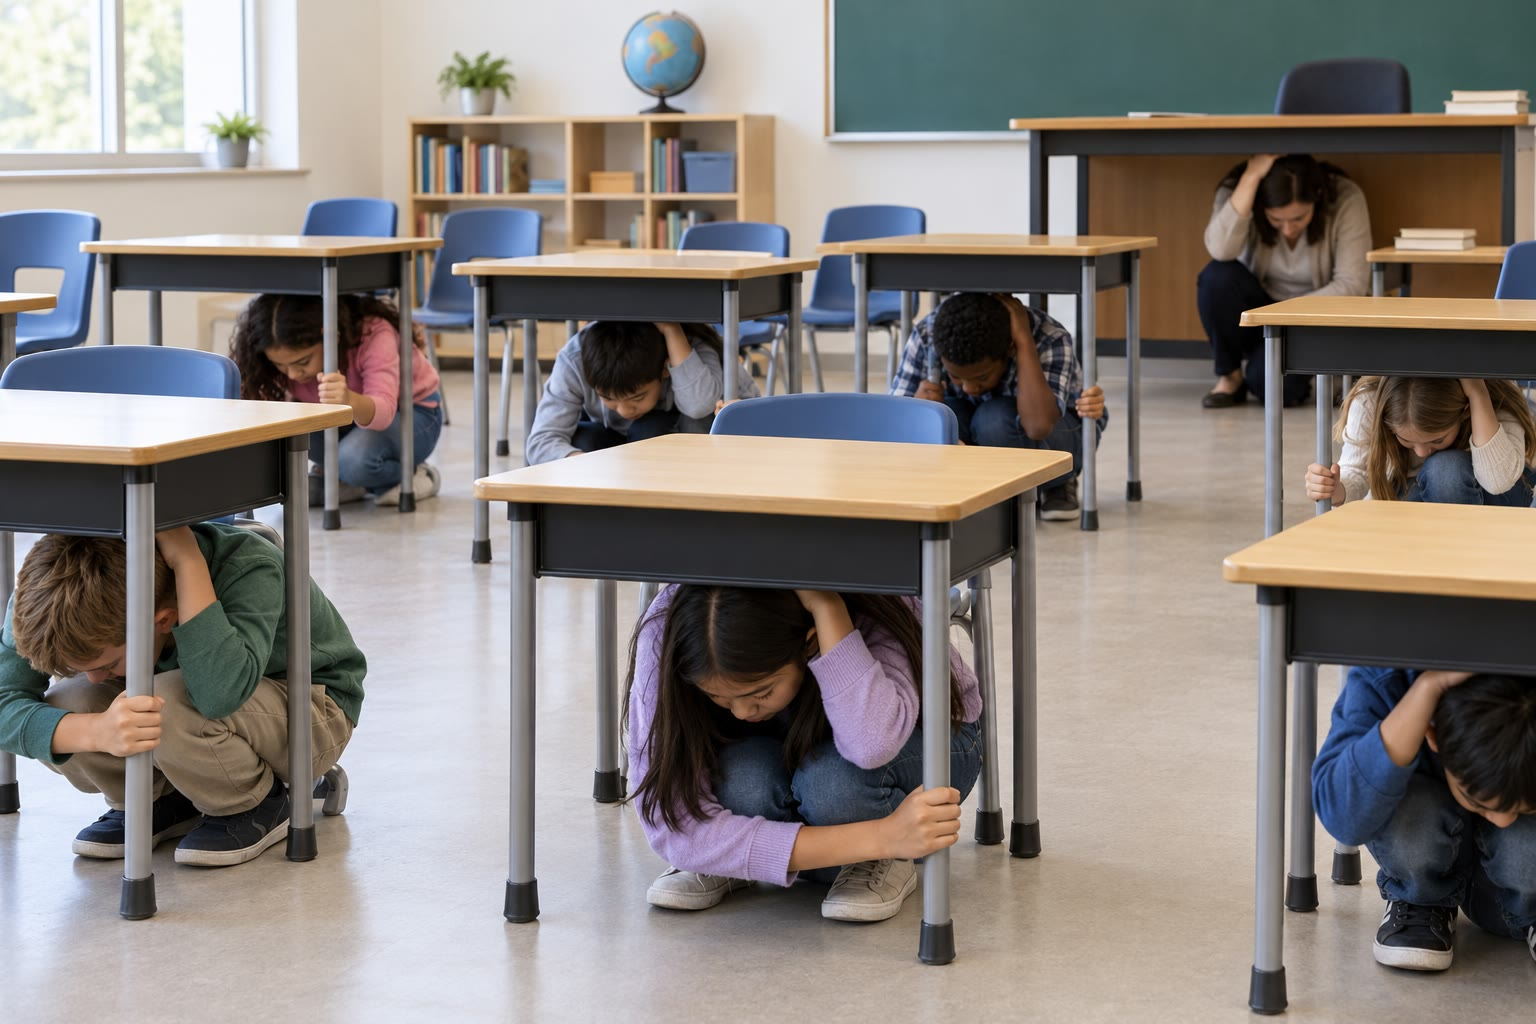
\includegraphics[width=0.55\linewidth]{images/book1/ai/g4-earthquake-drill.jpg}

{\small \omterm{def:g4:volcanoes-earthquakes-first-look:earthquake}{भूकंप} का अभ्यास: विद्यार्थी अपनी मेज़ों के नीचे ``झुको, ढको और पकड़े
रहो'' का अभ्यास करते हैं।}
\end{omfigure}

\section{अभ्यास}

\begin{exercise}[$\star$]\label{exo:g4:volcanoes-earthquakes-first-look:1}
\omterm{def:g4:volcanoes-earthquakes-first-look:eruption}{लावा}, राख या गैस? (क) ढलान पर बहती दमकती पिघली \omterm{def:g3:stones-pebbles-sand:rock}{चट्टान} की एक \omterm{def:g1:landscapes-around-us:water}{नदी};
(ख) आसमान में उड़ाए गए \omterm{def:g3:stones-pebbles-sand:rock}{चट्टान} के नन्हे टुकड़े, जो धूसर \omterm{def:g4:clouds-rain-snow:precipitation}{हिम} की तरह वापस गिरते हैं;
(ग) कुछ अदृश्य, जो राख के साथ \omterm{def:g4:volcanoes-earthquakes-first-look:volcano}{ज्वालामुखी} से निकल भागता है।
\end{exercise}

\begin{exercise}[$\star$]\label{exo:g4:volcanoes-earthquakes-first-look:2}
\omterm{def:g4:volcanoes-earthquakes-first-look:earthquake}{भूकंप} क्या है? क्या वह घंटों चलता है, या सेकंडों?
\end{exercise}

\begin{exercise}[$\star$]\label{exo:g4:volcanoes-earthquakes-first-look:3}
तीनों क़दमों को क्रम में लगाओ: पकड़े रहो; झुको; ढको।
\end{exercise}

\begin{exercise}[$\star$]\label{exo:g4:volcanoes-earthquakes-first-look:4}
पृष्ठ~\pageref{fig:g4:volcanoes-earthquakes-first-look:map} के \omterm{def:g2:drawing-to-map:map}{मानचित्र} पर, ज़्यादातर
\omterm{def:g4:volcanoes-earthquakes-first-look:volcano}{ज्वालामुखी} किस \omterm{def:g2:water-on-earth:ocean}{महासागर} के चारों ओर हैं?
\end{exercise}

\begin{exercise}[$\star$]\label{exo:g4:volcanoes-earthquakes-first-look:5}
सही या ग़लत? (क) ज़्यादातर \omterm{def:g4:volcanoes-earthquakes-first-look:earthquake}{भूकंप} इतने छोटे होते हैं कि महसूस नहीं होते। (ख) \omterm{def:g4:volcanoes-earthquakes-first-look:eruption}{लावा}
हमेशा के लिए द्रव रहता है। (ग) जब ज़मीन काँपे, तो सबसे सुरक्षित काम है बाहर
भागना।
\end{exercise}

\begin{exercise}[$\star$]\label{exo:g4:volcanoes-earthquakes-first-look:6}
पृष्ठ~\pageref{fig:g4:volcanoes-earthquakes-first-look:volcano} पर \omterm{def:g4:volcanoes-earthquakes-first-look:volcano}{ज्वालामुखी} का चित्र देखो।
पिघली \omterm{def:g3:stones-pebbles-sand:rock}{चट्टान} कहाँ से आती है? वह कहाँ से बाहर निकलती है?
\end{exercise}

\begin{exercise}[$\star\star$]\label{exo:g4:volcanoes-earthquakes-first-look:7}
\omterm{def:g2:drawing-to-map:map}{मानचित्र} पर ढूँढो: (क) अमेरिका महाद्वीपों का एक देश जिसकी पूरी लंबाई के साथ
बहुत-से \omterm{def:g4:volcanoes-earthquakes-first-look:volcano}{ज्वालामुखी} हैं; (ख) प्रशांत \omterm{def:g2:water-on-earth:ocean}{महासागर} के बीच में द्वीपों का एक समूह,
\omterm{def:g4:volcanoes-earthquakes-first-look:volcano}{ज्वालामुखियों} वाला, जो वलय पर नहीं है।
\end{exercise}

\begin{exercise}[$\star\star$]\label{exo:g4:volcanoes-earthquakes-first-look:8}
साल में लगभग 141 बड़े \omterm{def:g4:volcanoes-earthquakes-first-look:earthquake}{भूकंप} होते हैं। यह एक महीने में लगभग कितने हुए? (एक साल में
12 महीने होते हैं; पूर्ण संख्या में जवाब दो।)
\end{exercise}

\begin{exercise}[$\star\star$]\label{exo:g4:volcanoes-earthquakes-first-look:9}
हर 4 में से लगभग 3 बहुत बड़े \omterm{def:g4:volcanoes-earthquakes-first-look:earthquake}{भूकंप} प्रशांत के चारों ओर के वलय में होते हैं।
20 बहुत बड़े \omterm{def:g4:volcanoes-earthquakes-first-look:earthquake}{भूकंपों} में से तुम वलय में लगभग कितनों की अपेक्षा करोगे? और उसके
बाहर कितनों की?
\end{exercise}

\begin{exercise}[$\star\star$]\label{exo:g4:volcanoes-earthquakes-first-look:10}
\omterm{def:g4:volcanoes-earthquakes-first-look:earthquake}{भूकंप} के अभ्यास के दौरान लियो भागकर कक्षा के दरवाज़े की चौखट में खड़ा हो जाता है।
उसे इसके बदले क्या करना चाहिए था, और क्यों?
\end{exercise}

\begin{exercise}[$\star\star\star$]\label{exo:g4:volcanoes-earthquakes-first-look:11}
\omterm{def:g2:drawing-to-map:map}{मानचित्र} के 1\,214 \omterm{def:g4:volcanoes-earthquakes-first-look:volcano}{ज्वालामुखियों} में से 837 प्रशांत के चारों ओर के वलय में हैं।
कितने उसके बाहर हैं? क्या ``लगभग 3 में से 2'' वलय के हिस्से का अच्छा वर्णन है?
(संकेत: 1\,200 का दो-तिहाई कितना है?)
\end{exercise}
